\documentclass[11pt,a4paper,twoside,pdf]{article}

% Encoding and typography
\usepackage[T1]{fontenc}
\usepackage[utf8]{inputenc}
\usepackage{mathpazo}
\usepackage{braket}

% Mathematics
\usepackage{amsmath, amssymb, amsfonts}
\usepackage{bm}
\usepackage[mathscr]{euscript}

% Figures
\usepackage{graphicx}
\graphicspath{{./}{../figures/}}
\usepackage{float}
\usepackage{subcaption}

% Tables and utilities
\usepackage{multirow}
\usepackage{rotating}
\usepackage{array}
\usepackage{booktabs}
\usepackage{xspace}

% Additional symbols
\usepackage{eurosym}
\usepackage{bbding}
\usepackage{pifont}

% Other
\usepackage{soul}
\usepackage{color}
\usepackage{latexsym}
\usepackage{xtab}

% Hyperlinks
\usepackage[colorlinks=true,urlcolor=blue,linkcolor=blue,citecolor=blue]{hyperref}

% Equation numbering
\numberwithin{equation}{section}

% Margins
\usepackage[top=2.88cm,bottom=2.97cm,left=2.95cm,right=2.95cm]{geometry}

% Language
\usepackage[english]{babel}

% Headers
\usepackage{fancyhdr}

% Theorems
\newtheorem{theorem}{Theorem}[section]
\newtheorem{corollary}{Corollary}[theorem]
\newtheorem{lemma}[theorem]{Lemma}

% Custom commands
\newcommand{\dis}{\displaystyle}

\linespread{1.05}

\begin{document}

% Title page %%%%%%%%%%%%%%%%%%%%%%%%%%%%%%%%%%%%%%%%%%%%%%%%%%%%%%%%%%%%%%%%%%%

\pagestyle{empty}

\noindent
\begin{tabular}{r}

\includegraphics[width=8.8cm]{escudoUGRmonocromo.png} \\[-1.8ex]
\hspace{31mm}\vspace{-8mm}
\begin{tabular}{c}
\hline\\[-1ex]\hskip-2mm
{\bf Faculty of Sciences}\hspace{18mm}
\end{tabular}
\end{tabular}

\large
\vspace{10mm}
\hspace{25mm}
\begin{tabular}{l}
MASTER'S DEGREE IN PHYSICS: RADIATION, NANOTECHNOLOGY,\\
PARTICLES AND ASTROPHYSICS
\end{tabular}

\vspace{5mm}
\hspace{25mm}
\begin{tabular}{l}
MATHEMATICAL AND NUMERICAL COMPLEMENTS
\\[1.5ex]
\LARGE\bf DIFFUSION MONTE CARLO AND \\
\LARGE\bf THE HARMONIC ATOM
\end{tabular}

\hspace{2mm}
\begin{tabular}{l}
By:\\
{\bf A. S. Amari Rabah}
\end{tabular}

\begin{abstract}
The ground-state energy of a system of bosonic particles in a harmonic potential is
studied numerically as a function of the interaction parameter $\beta^2$ and the number
of particles $N$, using the Diffusion Monte Carlo (DMC) method. Both the basic
formulation without importance sampling and its guided version using the Trotter
approximation are considered.
\end{abstract}

% Table of contents %%%%%%%%%%%%%%%%%%%%%%%%%%%%%%%%%%%%%%%%%%%%%%%%%%%%%%%%%%%%

\tableofcontents

% Main text %%%%%%%%%%%%%%%%%%%%%%%%%%%%%%%%%%%%%%%%%%%%%%%%%%%%%%%%%%%%%%%%%%%%

\pagestyle{fancy}
\fancyhead[RO,LE]{\leftmark}
\fancyhead[LO,RE]{\thepage}
\fancyfoot{}

\newpage

\section{Introduction}

Starting from the time-dependent Schrödinger equation with a reference energy $E_T$

\begin{equation}
    i\hbar \frac{\partial \Psi (\mathbf{r}, t) }{\partial t} = (\hat{H} - E_T) \Psi (\mathbf{r}, t),
\end{equation}

and passing to imaginary time $\tau = it/\hbar$, one obtains

\begin{equation}
    \frac{\partial \Psi (\mathbf{r}, \tau) }{\partial \tau} = -(\hat{H} - E_T) \Psi (\mathbf{r}, \tau)
\label{ESimag}
\end{equation}

where $\mathbf{r}$ is the position vector of the particles in configuration space,
$\mathbf{r} \in \Omega$, $\mathbf{r} = (\mathbf{r}_1, \mathbf{r}_2, \cdots, \mathbf{r_N})$.
Equation~\ref{ESimag} has the \textit{symbolic} solution

$$
    \Psi (\mathbf{r}, \tau) = e^{-(\hat{H}-E_T)\tau} \Psi (\mathbf{r}, \tau=0).
$$

Assuming the initial wavefunction can be expanded in eigenfunctions of the
Hamiltonian, $\hat{H}\psi_n = E_n\psi_n$, with energies $E_n$ in increasing order
($E_1 < E_2 < \cdots < E_n$),

$$
    \Psi (\mathbf{r}, \tau) = \sum_{n} e^{-(E_n-E_T)\tau} \braket{\psi_n|\Psi_0} \psi_n.
$$

At large imaginary times the ground state dominates, so

$$
    \lim_{\tau \to \infty} \Psi(\mathbf{r}, \tau) \to e^{-(E_0-E_T)\tau} \braket{\psi_0|\Psi_0} \psi_0.
$$

The main difficulty in applying the time-evolution operator is computing the
exponential of the Hamiltonian, since the kinetic $\hat{T}$ and potential $\hat{V}$
operators do not generally commute:

$$
    \ket{\Psi(\mathbf{r}, \tau)} = e^{-(\hat{H}-E_T)\tau} \ket{\Psi(\mathbf{r}, 0)}.
$$

The \textit{short-time approximation} is therefore applied, computing the state at
each small time step $\Delta \tau$:

$$
    \ket{\Psi(\mathbf{r}, \tau + \Delta \tau)} = e^{-(\hat{H}-E_T)\Delta \tau} \ket{\Psi(\mathbf{r}, \tau)}.
$$

Applying the Trotter approximation to the time-evolution operator~\cite{kalos2008monte}:

\begin{equation}
    e^{-(\hat{H}-E_T)\Delta \tau} = e^{-(\hat{V}-E_T)\Delta \tau/2}e^{-\hat{T}\Delta \tau}e^{-(\hat{V}-E_T)\Delta \tau /2} + \mathcal{O} (\Delta \tau^3).
\label{Trotter}
\end{equation}

In the position representation the state at time $\tau + \Delta \tau$ is

$$
    \Psi(\mathbf{r}, \tau + \Delta \tau) = \braket{\mathbf{r}|\Psi(\tau + \Delta \tau)} =  \braket{\mathbf{r}| e^{-(\hat{H}-E_T)\Delta \tau} | \Psi( \tau)}.
$$

Using the resolution of identity in $\mathbf{r'}$,

$$
    \Psi(\mathbf{r}, \tau + \Delta \tau) =\int_{\mathbf{r'}} \braket{\mathbf{r}| e^{-(\hat{H}-E_T)\Delta \tau} | \mathbf{r'}} \Psi(\mathbf{r'}, \tau ) d\mathbf{r'}.
$$

Inserting resolutions of identity in $\mathbf{r''}$ and $\mathbf{r'''}$
with the approximation~\ref{Trotter},

$$
    \Psi(\mathbf{r}, \tau + \Delta \tau) =
    \int_{\mathbf{r'}} \int_{\mathbf{r''}} \int_{\mathbf{r'''}}
    \braket{\mathbf{r}| e^{-(\hat{V}-E_T)\Delta \tau/2} | \mathbf{r''}}
$$
$$
    \cdot \braket{\mathbf{r''}| e^{-\hat{T}\Delta \tau} | \mathbf{r'''}}
    \braket{\mathbf{r'''}|e^{-(\hat{V}-E_T)\Delta \tau/2} | \mathbf{r'}}
    \Psi(\mathbf{r'}, \tau )
    \,d\mathbf{r'} d\mathbf{r''} d\mathbf{r'''}.
$$

Computing each factor individually:

\begin{itemize}
    \item $\braket{\mathbf{r}| e^{-(\hat{V}-E_T)\Delta \tau/2} | \mathbf{r''}} = e^{-(\hat{V}(\mathbf{r''})-E_T)\Delta\tau/2} \delta(\mathbf{r-r''})$,
    \item $\braket{\mathbf{r'''}|e^{-(\hat{V}-E_T)\Delta \tau/2} | \mathbf{r'}} = e^{-(\hat{V}(\mathbf{r'})-E_T)\Delta\tau/2} \delta(\mathbf{r'''-r'})$,
    \item The kinetic energy operator is $-\Delta \tau \hat{T} = \frac{\Delta \tau \hbar^2}{2m} \nabla^2$, so:

    $\braket{\mathbf{r''}| e^{-\hat{T}\Delta \tau} | \mathbf{r'''}} = \dfrac{1}{(4\pi D \Delta \tau)^{N/2}} \exp\!\left(-\dfrac{(\mathbf{r''} - \mathbf{r'''})^2}{4\pi D \Delta \tau}\right)$

    where $D=\hbar^2/2m$ and $\sigma^2 = 2D\Delta \tau$.
\end{itemize}

The total state evolution is therefore

\begin{equation}
    \Psi(\mathbf{r}, \tau + \Delta \tau) = \frac{1}{(2\pi \sigma^2)^{N/2}} \int_{\mathbf{r'}} e^{-\frac{(\mathbf{r} - \mathbf{r'})^2}{2\sigma^2}} e^{-\Delta \tau /2 \left[ \hat{V}(\mathbf{r}) +  \hat{V}(\mathbf{r'}) - 2E_T \right] } \Psi (\mathbf{r'}, \tau) \,d \mathbf{r'}.
\label{Psitotal}
\end{equation}


\subsection{Diffusion Monte Carlo}
\label{DMC}

In practice, when the number of particles $N$ is large the integral in~\ref{Psitotal}
is impossible to evaluate directly. A stochastic interpretation based on Monte Carlo
methods, known as \textit{Diffusion Monte Carlo} (DMC)~\cite{hammond1994monte}, is
therefore employed.

In the DMC method the wavefunction is not represented as a continuous function
but by a population of $M$ fictitious particles called \textit{walkers}. Each walker
corresponds to a point in the configuration space of the system, i.e.\ we write $\Psi$ as

$$
    \Psi(\mathbf{r}, \tau) = \sum_{n=0}^M \delta(\mathbf{r} - \mathbf{r_i}(\tau)).
$$

The density of walkers in configuration space is proportional to the value of the
wavefunction. The evolution equation takes the general form

\begin{center}
new state $=$ propagator $\times$ old state.
\end{center}

In the Monte Carlo context the propagator is interpreted as a probability distribution
governing the transition of a walker from its current position to a new one. The
propagator separates into two main contributions: diffusion and branching.

The Gaussian term of the propagator describes a diffusion process. At each time
step each walker moves randomly according to a normal distribution — the new
position is obtained by adding a Gaussian random displacement to the previous one.
This represents the effect of the kinetic energy and can be interpreted as a random
walk through configuration space.

The potential-dependent term does not directly modify the walker's position
but its statistical weight\footnote{In the simulation the multiplicative factor $m_i$
is taken as the integer part of the weight $w_i$ plus a uniform random number between
0 and 1 to avoid bias.}. This factor determines the probability of survival or
reproduction of each walker. When the local potential is low, the walker is more
likely to be replicated. In regions of high potential, walkers tend to disappear;
the process thus acts as a natural-selection mechanism that favours low-energy
regions\footnote{For potentials that diverge to $-\infty$, walkers reproduce
indefinitely and a special treatment is required in DMC.}.

The Langevin equation associated with the Fokker–Planck equation~\ref{ESimag}
is~\cite{van1992stochastic}

$$
    d \mathbf{r} (\tau) = \sqrt{2D}\, d \mathbf{W} (\tau),
$$

where $d\mathbf{W}$ is a Wiener process. In discrete form the process is Markovian
and the walker positions obey

\begin{equation}
    \mathbf{r_{n+1}} = \mathbf{r_n} + \sqrt{2D\Delta \tau}\, \boldsymbol{\eta_n}
\label{langevindmcpuro}
\end{equation}

where $\boldsymbol{\eta_n} \sim \mathcal{N}(0, 1)$, and at each time step walkers
are multiplied by the weight
$w_n = \exp \left[ - \Delta \tau / 2 \cdot ( V(\mathbf{r_n}) + V(\mathbf{r_{n+1}})- 2E_T) \right]$.


\subsubsection{Energy estimation}

Two approaches exist for estimating the ground-state energy from $E_T$. Integrating
expression~\ref{Psitotal} over all walker positions $\mathbf{r}$ gives an estimate
of the population $M(\tau)$:

$$
    M(\tau + \Delta \tau) = \int_{\mathbf{r}} \Psi(\mathbf{r}, \tau + \Delta \tau)\, d\mathbf{r} = e^{-(E_0 - E_T)\Delta \tau} M(\tau).
$$

The first option is to keep a population of walkers that evolves with time
(via the weights) and hold $E_T$ constant, so iterating the relation above gives

$$
    E_0 \approx E_T - \frac{1}{\tau} \ln \frac{M(\tau)}{M(0)},
$$

or equivalently by averaging several measurements of

$$
    E_0 \approx E_T + \frac{1}{\Delta \tau} \ln \frac{M(\tau)}{M(\tau + \Delta \tau)}.
$$

\newpage
In this scheme the population at the next time step is the previous population with
each walker weighted by its statistical weight, which requires a population-control
method to prevent runaway growth. The alternative is to hold the population
constant at $M_0$ and let $E_T(\tau)$ vary:

$$
    \frac{d M(\tau)}{d\tau} = \int_{\mathbf{r}} \frac{\partial \Psi (\mathbf{r}, \tau)}{\partial \tau}\, d\mathbf{r} =  \int_{\mathbf{r}} (\hat{T} + \hat{V} - E_T (\tau)) \Psi (\mathbf{r}, \tau)\, d\mathbf{r} = \int_{\mathbf{r}} (E_0 - E_T(\tau)) \Psi (\mathbf{r}, \tau)\, d\mathbf{r} = 0.
$$

The kinetic term $\int_{\mathbf{r}} \nabla \cdot (\nabla \Psi(\mathbf{r}, \tau))\, d\mathbf{r}$
is evaluated at the boundaries of configuration space; for a wavefunction that decays
sufficiently fast it can be neglected. This is valid for the harmonic potential
considered here.

The condition on $E_T$ is

$$
    E_T (\tau)= \frac{\int \hat{V} (\mathbf{r}) \Psi(\mathbf{r},  \tau)\, d\mathbf{r}}{\int  \Psi(\mathbf{r},  \tau)\, d\mathbf{r}} = \braket{\hat{V}}_{\Psi (\tau)},
$$

adjusted dynamically at each time step as

$$
    E_T (\tau + \Delta \tau) = \braket{\hat{V}}_{\Psi (\tau)}.
$$

The ground-state energy $E_0$ is estimated as the time average of $E_T(\tau)$.

To avoid both the runaway-growth problem and the fixed-population bias, a
mixed scheme is used in which the population is allowed to \emph{oscillate} around a
target value $M_0$:

$$E_T(\tau + \Delta \tau) = \braket{\hat{V}}_{\Psi(\tau)} + \frac{\gamma}{\Delta \tau} \ln \left( \frac{M_0}{M(\tau)} \right),$$

where $\gamma$ is a small damping factor. If $M(\tau)$ falls below $M_0$,
the term becomes positive, raising $E_T$ and encouraging walker replication;
if the population exceeds $M_0$, $E_T$ decreases and walkers are annihilated.


\subsection{Importance Sampling}
\label{IS}

Although the DMC method largely overcomes the curse of dimensionality, it
introduces other problems. Walkers explore configuration space by free diffusion,
frequently visiting regions where the wavefunction is nearly zero and wasting
computational effort on regions irrelevant to the ground state. This causes the
statistical variance to grow rapidly, leading to large fluctuations.

To improve efficiency, a trial (guide) wavefunction $\Psi_T(\mathbf r)$ that
approximates the ground state is introduced. Instead of sampling $\Psi$ directly,
one works with the function

\begin{equation}
f(\mathbf r,\tau)
=
\Psi_T(\mathbf r)\Psi(\mathbf r,\tau).
\end{equation}

Substituting this definition into the evolution equation~\ref{ESimag} yields a
Fokker–Planck equation

\begin{equation}
\frac{\partial f}{\partial \tau}
=
D \nabla^2 f
-
\nabla \cdot \left( \mathbf F(\mathbf r) f \right)
-
\left[E_L(\mathbf r)-E_T\right] f,
\end{equation}

where $\mathbf F(\mathbf r) = 2D \nabla \ln \Psi_T(\mathbf r)$ is the drift force
and $E_L(\mathbf r) = \frac{\hat H \Psi_T(\mathbf r)}{\Psi_T(\mathbf r)}$ is the
local energy. The kinetic term now becomes a drift-diffusion process and the
branching term depends only on the local energy. The Trotter approximation for the
state evolution reads

\begin{equation}
\begin{split}
    f(\mathbf{r}, \tau + \Delta \tau) = \int_{\mathbf{r'}} \frac{1}{(2\pi \sigma^2)^{N/2}} \exp \left( -\frac{1}{2\sigma^2} \left[ \mathbf{r} - \mathbf{r'} -\mathbf{F}(\mathbf{r'}) \Delta \tau \right]^2 \right) \\
    \cdot \exp \left( \Delta \tau \left[ E_T - \frac{1}{2}( E_L(\mathbf{r}) + E_L(\mathbf{r'})) \right] \right) f(\mathbf{r'}, \tau) \,d\mathbf{r'}.
\end{split}
\end{equation}

With this transformation walkers no longer perform a pure random walk; instead
they \textit{feel} a drift towards regions where $\Psi_T$ is large. Sampling is
concentrated in the physically relevant regions of configuration space, the
statistical variance is drastically reduced, and the branching process depends
on the local energy rather than the bare potential.

The discrete Langevin equation guiding the walkers is

\begin{equation}
\mathbf r_{n+1}
=
\mathbf r_n
+
\mathbf F(\mathbf r_n)\Delta\tau
+
\sqrt{2D\Delta\tau}\,\boldsymbol\eta_n,
\notag
\end{equation}

and walkers are multiplied by the weights
$w_n = \exp\left[-\Delta\tau / 2 \left(E_L(\mathbf r_{n}) + E_L(\mathbf r_{n+1}) - 2E_T\right)\right]$.

Finally, the ground-state energy $E_0$ is estimated as the mean local energy
with respect to $f$. Using the Hermiticity of the Hamiltonian:

$$
    \braket{E_L}_{f} = \frac{\int f E_L\, dr}{\int f\, dr} = \frac{ \int \Psi_T \Psi_0 \frac{\hat{H} \Psi_T }{\Psi_T}\, dr}{ \int \Psi_T \Psi_0\, dr }
    = \frac{ \int \Psi_0 \hat{H} \Psi_T\, dr}{  \int \Psi_T \Psi_0\, dr }
$$
$$
    = \frac{ \int \Psi_T \hat{H} \Psi_0\, dr}{  \int \Psi_T \Psi_0\, dr } = \frac{ \int \Psi_T E_0 \Psi_0\, dr}{  \int \Psi_T \Psi_0\, dr } = E_0.
$$

The population-control update is

$$E_T(\tau + \Delta \tau) = \braket{E_L}_{f(\tau)} + \frac{\gamma}{\Delta \tau} \ln \left( \frac{M_0}{M(\tau)} \right).$$


\section{The Harmonic Atom}

We consider particles moving in three-dimensional space and interacting through
the Hamiltonian

\begin{equation}
    \hat{H} = -\frac{1}{2} \sum_{k=1}^N \nabla_{\mathbf{r}_k}^2
    + \frac{1}{2} \sum_{k=1}^N \mathbf{r}_k^2  -\frac{\beta^2}{2N} \sum_{l>k=1}^N |\mathbf{r}_{k} - \mathbf{r}_l|^2 \,,
\label{hamiltonianoatomoarmonico}
\end{equation}

with $0 \leq \beta^2 <1$. The analytical ground-state energy is~\cite{armstrong2012quantum}

\begin{equation}
    E_{\mathrm{exact}} = \frac{3}{2} \left[ 1 + (N-1) \sqrt{1 - \beta^2}\right].
\label{Eexact}
\end{equation}


\subsection{Pure Diffusion Monte Carlo}

Since the potential is harmonic, walkers are initialised from a Gaussian centred
at the origin, $\mathbf r_i(0)\sim \mathcal N(0, D)$. Because this initialisation is
arbitrary and may not represent the true ground state, the first steps are discarded
— a procedure known as thermalisation or \textit{burn-in}~\cite{newman1999monte}.
Here the thermalisation time is set to \texttt{0.3\,*\,Nsteps}, where $Nsteps$ is
the total number of time steps $\Delta \tau$.

At each time step $\Delta\tau$ walkers evolve by free diffusion via the Langevin
equation $\mathbf{r_{n+1}} = \mathbf{r_n} + \sqrt{2D\Delta \tau}\,\boldsymbol{\eta_n}$
and are multiplied by the weight
$w_n = \exp \left[ - \Delta \tau / 2 \cdot ( V(\mathbf{r_n}) + V(\mathbf{r_{n+1}})- 2E_T) \right]$.

The total number of walkers is regulated dynamically by adjusting $E_T$ via
$E_T(\tau+\Delta\tau) = \braket{\hat{V}}_{\Psi(\tau)} + \frac{1}{\Delta\tau} \ln\frac{M_0}{M(\tau)}$,
where $M_0$ is the target population. Once the stationary regime is reached, the
time average of $E_T$ provides an estimate of the ground-state energy.


\subsubsection{Results}

Figure~\ref{E0DMCpuro} shows the numerical results obtained with the pure DMC
method described in section~\ref{DMC}, together with the analytical solution
equation~\ref{Eexact}, for several values of the particle number $N$.

In all cases the ground-state energy decreases monotonically with $\beta^2$,
reflecting the weakening of the confinement as the interaction strength increases.
The small deviations can be attributed to statistical fluctuations in the sampling
and, to a lesser extent, to the discretisation error.

For $N=2$, $N=5$, and $N=10$ there is overall agreement between the numerical
results and the analytical solution across the full range of $\beta^2$. For $N=20$,
however, a more pronounced discrepancy appears, especially at small and intermediate
values of $\beta^2$, where DMC tends to overestimate the ground-state energy. This
deviation originates in the growth of configuration space with particle number,
which makes efficient sampling by free diffusion increasingly difficult. A significant
fraction of walkers explore low-probability regions, raising the variance. The effects
of finite population control and the discrete time step are also amplified in larger
systems.

This motivates the use of importance sampling to obtain accurate results for
systems with a large number of particles or strong interactions.

\begin{figure}[H]
    \centering
    \begin{minipage}[t]{0.48\textwidth}
        \centering
        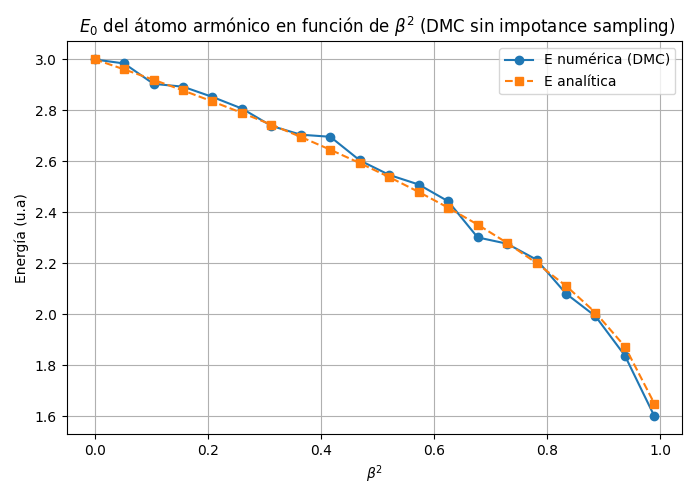
\includegraphics[width=\linewidth, height=5cm]{E0DMCPuroN2.png} \\[2pt]
        \small (a) $N = 2$.
    \end{minipage}
    \hfill
    \begin{minipage}[t]{0.48\textwidth}
        \centering
        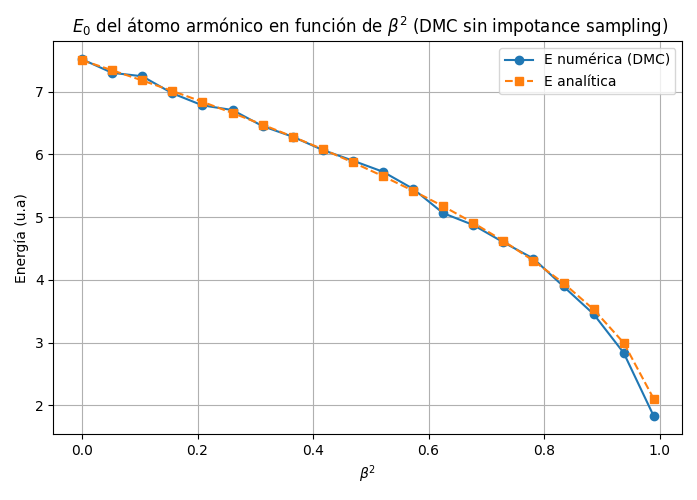
\includegraphics[width=\linewidth, height=5cm]{E0DMCPuroN5.png} \\[2pt]
        \small (b) $N = 5$.
    \end{minipage}

    \vspace{0.5cm}

    \begin{minipage}[t]{0.48\textwidth}
        \centering
        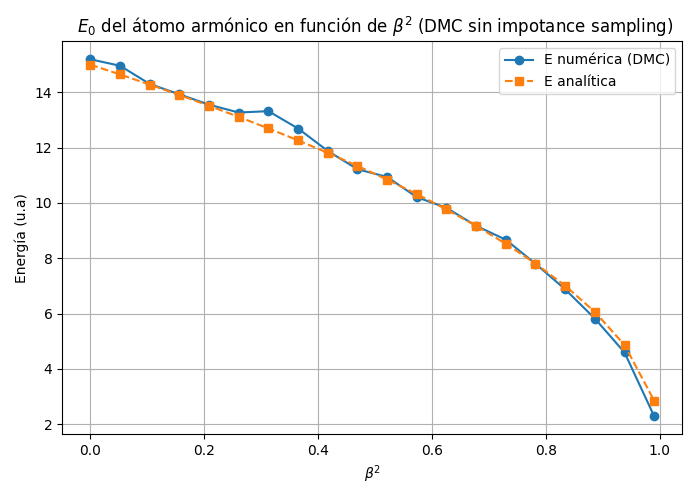
\includegraphics[width=\linewidth, height=5cm]{E0DMCPuroN10.png} \\[2pt]
        \small (c) $N = 10$.
    \end{minipage}
    \hfill
    \begin{minipage}[t]{0.48\textwidth}
        \centering
        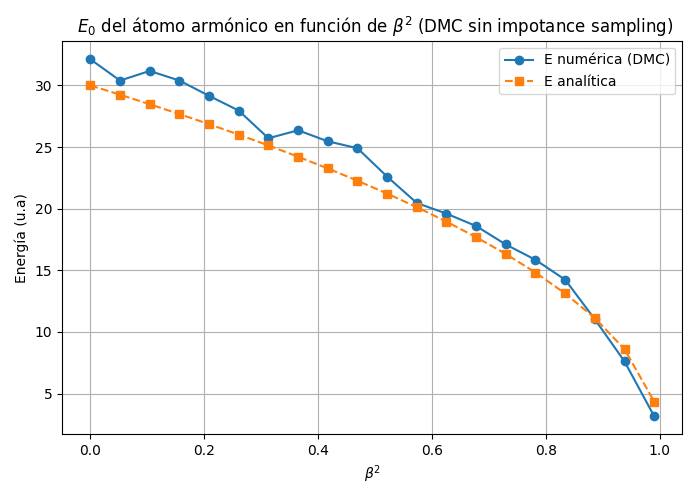
\includegraphics[width=\linewidth, height=5cm]{E0DMCPuroN20.png} \\[2pt]
        \small (d) $N = 20$.
    \end{minipage}

    \caption{Ground-state energy as a function of $\beta^2$ for different particle
    numbers. Atomic units; time step $\Delta \tau = 0.001$; $10^4$ steps; target
    population $2\cdot10^3$ walkers. Thermalisation: first $3\cdot10^3$ steps
    discarded. Results averaged over $10^3$ realisations.}
    \label{E0DMCpuro}
\end{figure}


\subsection{Importance Sampling}

As the trial wavefunction we take

\begin{equation}
    \ket{\Psi_\alpha} = \left( \frac{\alpha}{\pi} \right)^{\frac{3}{4}N}
    \exp \left( - \frac{\alpha}{2} (\mathbf{r}^2_1 + \cdots +  \mathbf{r}^2_N  )\right),
\end{equation}

which is the exact ground state of the non-interacting harmonic oscillator with
frequency $\omega=\alpha$. Walkers are also initialised from this distribution.
The drift force is

\begin{equation}
\mathbf F(\mathbf r)
=
2D \nabla \ln \Psi_\alpha(\mathbf r)
=
-2D\alpha
\left(
\mathbf r_1,\mathbf r_2,\ldots,\mathbf r_N
\right),
\end{equation}

which is a restoring force directed towards the origin of configuration space.
The Langevin equation becomes

\begin{equation}
\mathbf r_{n+1}
=
\mathbf r_n
-
2D\alpha\,\mathbf r_n \Delta\tau
+
\sqrt{2D\Delta\tau}\,\boldsymbol\eta_n.
\end{equation}

The local energy is

\begin{equation}
\begin{split}
E_L(\mathbf r) = \frac{\hat H \Psi_T(\mathbf r)}{\Psi_T(\mathbf r)} = \frac{3}{2}N\alpha + \frac12(1-\alpha^2)\sum_{k=1}^N r_k^2 - \frac{\beta^2}{2N}\sum_{l>k} r_{kl}^2 \\
= \frac{3}{2}N\alpha + \frac12(1-\alpha^2 - \beta^2)\sum_{k=1}^N r_k^2 + \frac{\beta^2}{2N} \left( \sum_{k=1}^N r_{k} \right)^2.
\end{split}
\end{equation}

With this transformation sampling becomes concentrated in the physically relevant
regions of configuration space, since the interacting ground state is expected to
resemble the non-interacting one.

The local energy depends on $\alpha$, which controls the width of the Gaussian
and the localisation of walkers. If $\Psi_\alpha$ were the exact ground state, the
local energy would be constant and the variance would vanish. In the
non-interacting limit ($\beta=0$), the exact value $\alpha=1$ gives a constant
$E_L=\frac{3}{2}N$. In the presence of interactions, the $\beta^2$ term modifies
the effective wavefunction width, requiring an adjustment of $\alpha$. Setting the
coefficient of $\sum_k r_k^2$ in the local energy to zero gives the near-optimal
estimate

\begin{equation}
\alpha_{\rm opt} \simeq \sqrt{1-\beta^2}.
\end{equation}


\newpage
\subsubsection{Results}

Figure~\ref{E0DMCIS} shows the numerical results obtained with IS-DMC described in
section~\ref{IS}, together with the analytical solution equation~\ref{Eexact},
for several values of $N$.

In all cases the agreement is excellent, even at large $\beta^2$ and large $N$.
The advantage is particularly striking at large particle numbers: an equivalent
deterministic calculation sampling $m$ points per dimension would cost
$\mathcal{O}(m^{3N})$ operations. For a modest $m=20$ and $N=10$ the cost is
$20^{30} \sim 10^{39}$; even at $10^{18}$ operations per second the computation
would exceed the age of the universe.

\begin{figure}[H]
    \centering
    \begin{minipage}[t]{0.48\textwidth}
        \centering
        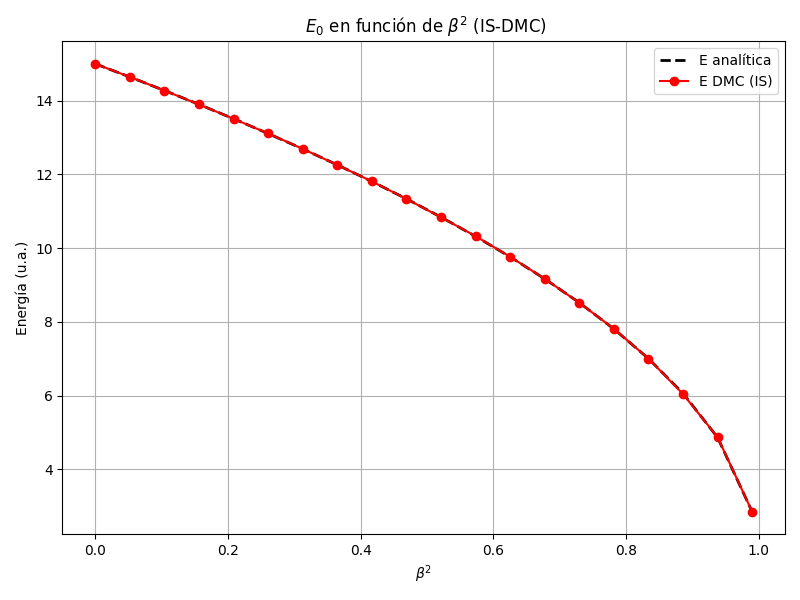
\includegraphics[width=\linewidth, height=5cm]{E0DMCISN10.png} \\[2pt]
        \small (a) $N = 10$.
    \end{minipage}
    \hfill
    \begin{minipage}[t]{0.48\textwidth}
        \centering
        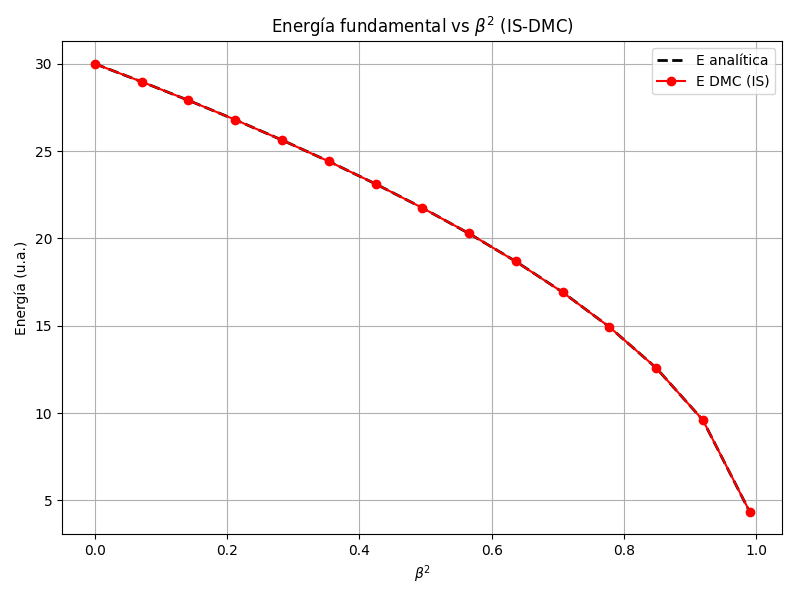
\includegraphics[width=\linewidth, height=5cm]{E0DMCISN20.png} \\[2pt]
        \small (b) $N = 20$.
    \end{minipage}

    \vspace{0.5cm}

    \begin{minipage}[t]{0.48\textwidth}
        \centering
        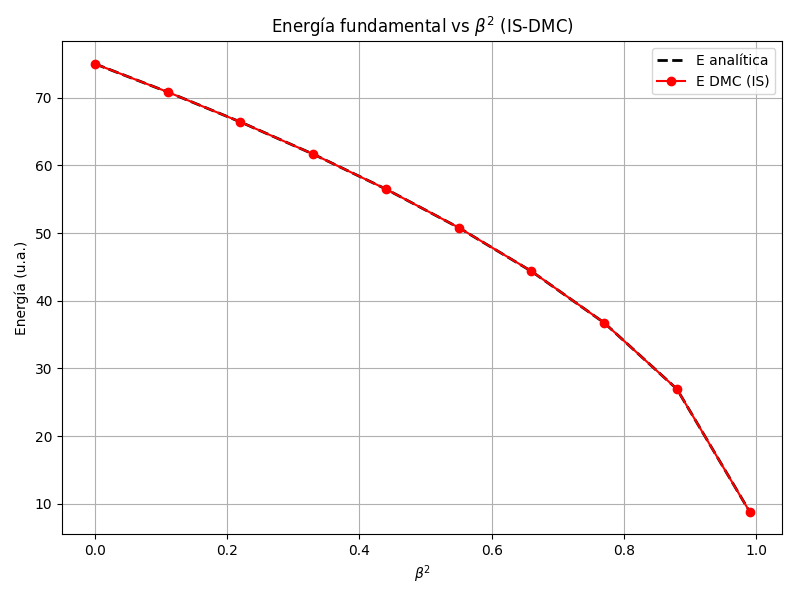
\includegraphics[width=\linewidth, height=5cm]{E0DMCISN50.png} \\[2pt]
        \small (c) $N = 50$.
    \end{minipage}
    \hfill
    \begin{minipage}[t]{0.48\textwidth}
        \centering
        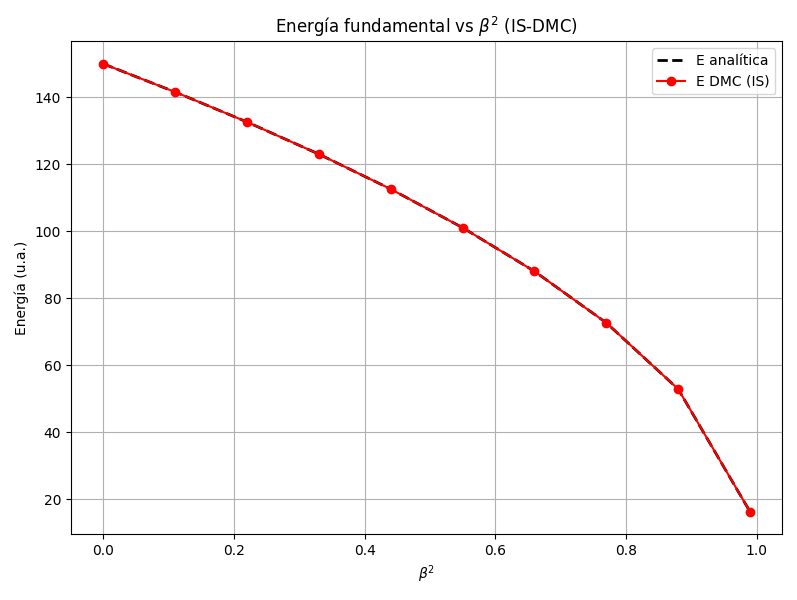
\includegraphics[width=\linewidth, height=5cm]{E0DMCISN100.png} \\[2pt]
        \small (d) $N = 100$.
    \end{minipage}

    \caption{Ground-state energy as a function of $\beta^2$ for different particle
    numbers. Atomic units; time step $\Delta \tau = 0.001$; $10^4$ steps; target
    population $2\cdot10^3$ walkers. Thermalisation: first $3\cdot10^3$ steps
    discarded. Results averaged over $10^3$ realisations.}
    \label{E0DMCIS}
\end{figure}


\newpage
\section{Conclusion}

The ground-state energy of a system of bosonic particles under a harmonic potential
has been studied numerically as a function of the interaction parameter $\beta^2$
and the particle number $N$, using the Diffusion Monte Carlo method, both in its
basic form (pure DMC) and with importance sampling via the Trotter approximation.

Pure DMC shows good agreement with the exact solution for small particle numbers.
As $N$ increases, however, the error grows noticeably due to inefficient sampling of
configuration space by free diffusion.

Importance sampling with a Gaussian trial wavefunction adds a drift term that
guides walkers towards the physically relevant regions and replaces the bare
potential with the local energy in the branching step. IS-DMC shows excellent
agreement with the analytical solution across the full range of $\beta^2$, even for
large particle numbers.

\newpage

\bibliographystyle{plain}
\bibliography{bibliografiaDMC}

\end{document}
